\documentclass[12pt, twoside]{article}
\usepackage[francais]{babel}
\usepackage[T1]{fontenc}
\usepackage[latin1]{inputenc}
\usepackage[left=5mm, right=5mm, top=5mm, bottom=5mm]{geometry}
\usepackage{float}
\usepackage{graphicx}
\usepackage{array}
\usepackage{multirow}
\usepackage{amsmath,amssymb,mathrsfs}
\usepackage{textcomp}
\pagestyle{empty}
\usepackage{soul}
\usepackage{eurosym}


\begin{document} 



\begin{flushleft}
NOM PRENOM: \ldots \ldots \ldots \ldots \ldots \ldots \ldots \ldots \ldots
 \end{flushleft}


\begin{center}
{\fbox{$6^{e}\ldots$ \qquad \qquad \textbf{\Large{Devoir surveill� 7 }}
\qquad \qquad 27/05/2011}}
\end{center}




\rule{19cm}{0,5 pt}

\medskip

\begin{tabular}{|l|c|c|c|}

 \hline
 
 \quad & un peu & beaucoup & pas du tout \\
\hline

J'ai r�vis� & \quad & \quad  & \quad \\

\hline

J'ai r�ussi & \quad & \quad & \qquad \\

\hline
\end{tabular}


\medskip


\begin{tabular}{|l|c|c|c|}
\hline

 \quad
 &


 acquis
  & 

 \begin{minipage}{25mm}
 en cours 
 
 d'acquisition
 \end{minipage}
                  
                  
& 


 non acquis

 \\

\hline


Division d�cimale pos�e & \quad & \quad & \quad \\


\hline

Tables de multiplication & \quad & \quad & \quad \\

\hline

Fractions �gales & \quad & \quad & \quad \\


\hline

 \begin{minipage}{4cm}
Prendre une fraction d'un nombre
\end{minipage}
 & \quad & \quad & \quad \\

\hline
\end{tabular}


\medskip


\rule{19cm}{0,5 pt}

\medskip


\ul{\textbf{Exercice 1:}} \textit{(3 points)}

\begin{enumerate}
  \item Donner l'�criture d�cimale: \quad  $\dfrac{41}{100}=
  \ldots \ldots$ \qquad \qquad $\dfrac{45}{3}=\ldots \ldots$ \qquad \qquad 
  $\dfrac{7}{5}=\ldots \ldots$
  \item Compl�ter les �galit�s suivantes: \quad $3 \times \dfrac{2}{3}= \ldots
  \ldots$ \qquad  \qquad $\dfrac{8}{11} \times \ldots \ldots = 8$ \qquad \qquad
  $5 \times \ldots \ldots = 13$
  
\end{enumerate}



\bigskip



\ul{\textbf{Exercice 2:}} \textit{(3 points)}

\enskip

Compl�ter les �galit�s suivantes en justifiant: 



\enskip



a) $\dfrac{3}{5}=\dfrac{\ldots \ldots}{15}$ \qquad \qquad 
b) $\dfrac{36}{24}=\dfrac{6}{\ldots \ldots}$ \qquad \qquad c) $2=\dfrac{\ldots
\ldots}{9}$ \qquad  \qquad d) $\dfrac{8}{18}=\dfrac{\ldots
\ldots}{9}=\dfrac{16}{\ldots \ldots}=\dfrac{0,16}{\ldots \ldots}$




\bigskip



\ul{\textbf{Exercice 3:}} \textit{(2 points)}


\enskip

Calculer en d�taillant les calculs: 

\enskip


a) $\dfrac{4}{3} \times 21$ = 
\ldots\ldots\ldots\ldots\ldots\ldots\ldots\ldots\ldots\ldots\ldots
\ldots\ldots\ldots\ldots\ldots\ldots\ldots\ldots\ldots\ldots\ldots 

\enskip

 b) $\dfrac{8}{20} \times 5 $ = \ldots\ldots\ldots\ldots\ldots\ldots\ldots\ldots\ldots\ldots\ldots
\ldots\ldots\ldots\ldots\ldots\ldots\ldots\ldots\ldots\ldots\ldots




\bigskip



\ul{\textbf{Exercice 4:}} \textit{(2 points)}


\begin{enumerate}
  \item Donner l'abscisse de A sous forme d'une fraction. \ldots \ldots \ldots
  \ldots
  \item Donner l'abscisse de C sous forme d'une fraction. \ldots \ldots \ldots
  \ldots  
  \item Placer sur la droite gradu�e, le point B d'abscisse $\dfrac{7}{5}$.
  \item Placer sur la droite gradu�e, le point R d'abscisse $1 + \dfrac{4}{5}$.
\end{enumerate}

\begin{center} 
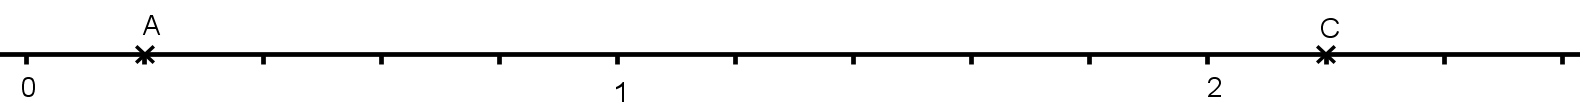
\includegraphics[width=14cm]{images/droite.png}
\end{center}

\bigskip



\ul{\textbf{Exercice 5:}} \textit{(3 points)}

\enskip

Jean a gagn� 1600 \euro. Il d�cide de donner $\dfrac{3}{8}$ de cette somme �
son fr�re Paul, $\dfrac{2}{5}$ de la somme � sa soeur Anne et il garde le reste.
Combien d'argents ont Paul, Anne et Jean?




\ldots \ldots \ldots \ldots \ldots \ldots \ldots \ldots \ldots \ldots \ldots
\ldots \ldots \ldots \ldots \ldots \ldots \ldots \ldots \ldots \ldots \ldots
\ldots \ldots \ldots \ldots \ldots \ldots \ldots \ldots \ldots \ldots
\ldots \ldots \ldots \ldots 


\ldots \ldots \ldots \ldots \ldots \ldots \ldots \ldots \ldots \ldots \ldots
\ldots \ldots \ldots \ldots \ldots \ldots \ldots \ldots \ldots \ldots \ldots
\ldots \ldots \ldots \ldots \ldots \ldots \ldots \ldots \ldots \ldots
\ldots \ldots \ldots \ldots 


\ldots \ldots \ldots \ldots \ldots \ldots \ldots \ldots \ldots \ldots \ldots
\ldots \ldots \ldots \ldots \ldots \ldots \ldots \ldots \ldots \ldots \ldots
\ldots \ldots \ldots \ldots \ldots \ldots \ldots \ldots \ldots \ldots
\ldots \ldots \ldots \ldots 


\ldots \ldots \ldots \ldots \ldots \ldots \ldots \ldots \ldots \ldots \ldots
\ldots \ldots \ldots \ldots \ldots \ldots \ldots \ldots \ldots \ldots \ldots
\ldots \ldots \ldots \ldots \ldots \ldots \ldots \ldots \ldots \ldots
\ldots \ldots \ldots \ldots 


\bigskip


\ul{\textbf{Exercice 6:}} \textit{(4 points)}

\enskip


\begin{tabular}{cc}
\begin{minipage}{14cm}
1. Observe le dessin puis �crire \textbf{une} phrase en utilisant le mot
``sym�trique''.

\ldots \ldots \ldots \ldots \ldots \ldots \ldots \ldots \ldots \ldots \ldots
\ldots \ldots \ldots \ldots \ldots \ldots \ldots \ldots \ldots \ldots \ldots
\ldots \ldots \ldots 



\ldots \ldots \ldots \ldots \ldots \ldots \ldots \ldots \ldots \ldots \ldots
\ldots \ldots \ldots \ldots \ldots \ldots \ldots \ldots \ldots \ldots \ldots
\ldots \ldots \ldots 


\end{minipage}
&
\begin{minipage}{4cm}
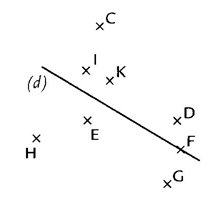
\includegraphics[width=4cm]{images/sym2.jpg}
\end{minipage} \\

\begin{minipage}{14cm}
2. 

\begin{enumerate}
  \item [a)] $B_1$ est-il le sym�trique du point A par rapport � (d)? Pourquoi?

\ldots \ldots \ldots \ldots \ldots \ldots \ldots \ldots \ldots \ldots \ldots
\ldots \ldots \ldots \ldots \ldots \ldots \ldots \ldots \ldots \ldots \ldots
 

\ldots \ldots \ldots \ldots \ldots \ldots \ldots \ldots \ldots \ldots \ldots
\ldots \ldots \ldots \ldots \ldots \ldots \ldots \ldots \ldots \ldots \ldots
    


\item [b)] $B_2$ est-il le sym�trique du point A par rapport � (d)? Pourquoi?

\ldots \ldots \ldots \ldots \ldots \ldots \ldots \ldots \ldots \ldots \ldots
\ldots \ldots \ldots \ldots \ldots \ldots \ldots \ldots \ldots \ldots \ldots
  


\ldots \ldots \ldots \ldots \ldots \ldots \ldots \ldots \ldots \ldots \ldots
\ldots \ldots \ldots \ldots \ldots \ldots \ldots \ldots \ldots \ldots \ldots


\item [c)] $B_3$ est-il le sym�trique du point A par rapport � (d)? Pourquoi?

\ldots \ldots \ldots \ldots \ldots \ldots \ldots \ldots \ldots \ldots \ldots
\ldots \ldots \ldots \ldots \ldots \ldots \ldots \ldots \ldots \ldots \ldots
 

\ldots \ldots \ldots \ldots \ldots \ldots \ldots \ldots \ldots \ldots \ldots
\ldots \ldots \ldots \ldots \ldots \ldots \ldots \ldots \ldots \ldots \ldots
  
\end{enumerate}

 



\end{minipage}
&
\begin{minipage}{5cm}
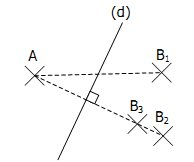
\includegraphics[width=5cm]{images/sym1.jpg}
\end{minipage} \\


\end{tabular}




3. 

\begin{enumerate}
  \item [a)] Construire sur la figure ci-dessous le sym�trique K du point C par
  rapport � la droite (d).
  \item [b)] Construire sur la figure ci-dessous le sym�trique T du point D par
  rapport � la droite (d).  
  \item[c)] Construire sur la figure ci-dessous le sym�trique Z du point F par
  rapport � la droite (d). 
\end{enumerate}

\begin{center}
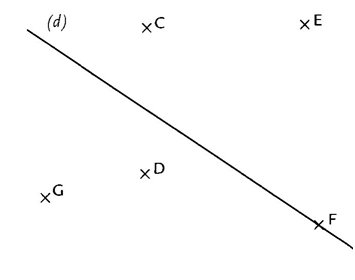
\includegraphics[width=7cm]{images/sym3.jpg}

\end{center}

\bigskip



\ul{\textbf{Exercice 7:}} \textit{(4 points)}

\enskip

Tracer le ou les axes de sym�trie (s'ils existent) et indique le nombre d'axes
sous chaque figure.

\medskip

\begin{tabular}{ccccc}
\begin{minipage}{25mm}
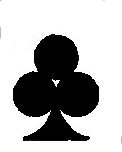
\includegraphics[width=2cm]{images/trefle.jpg}



\end{minipage}
&
\begin{minipage}{35mm}


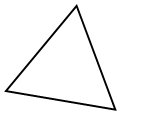
\includegraphics[width=3cm]{images/triangle.jpg}



\end{minipage}
&
\begin{minipage}{35mm}


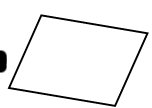
\includegraphics[width=3cm]{images/pgm.jpg}



\end{minipage}
&
\begin{minipage}{4cm}


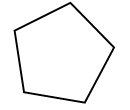
\includegraphics[width=3cm]{images/pentagone.jpg}



\end{minipage}
&
\begin{minipage}{4cm}


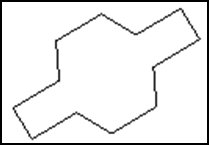
\includegraphics[width=3cm]{images/patate.jpg} 

\end{minipage} \\


\quad & \quad & \quad & \quad & \quad \\

\ldots \ldots axes
 

&


\ldots \ldots axes


&


\ldots \ldots axes


&


\ldots \ldots axes


&


\ldots \ldots axes


\\


\end{tabular}
\end{document}
